\section{Spectrum}

    % Let \(A\) be an integral \(\kk\)-algebra with \(\kk\) complete non-archimedean algebraically closed field.
    % For every \(\frakm \in \Spec A\), the absolute value on \(A/\frakm \cong \kk\) induces a multiplicative semi-norm on \(A\) by \(|f|_\frakm := |f \mod \frakm|\) for each \(f \in A\).

    % Suppose that we have an absolute value \(\|\cdot\|\) on \(\KK = \Frac A\) extending that on \(\kk\).
    % It induces a norm on \(A\) by restriction, denoted by \(\|\cdot\|_\eta\).

    % Then we can ``deform'' \(\|\cdot\|_\eta\) to \(|\cdot|_\frakm\) as follows:

    Let \(\kk\) be a spherically complete non-archimedean field which is algebraically closed and \(A = \kk[T]\).
    We want to consider the ``analytic structure'' on \(\mSpec A\).
    However, unlike the complex case, the set \(\mSpec A\) is totally disconnected with respect to the topology induced by the absolute value on \(\kk\) (\cref{prop:ultra-metric_space_is_totally_disconnected}).
    To overcome this difficulty, Berkovich uses multiplicative semi-norms to ``fill in the gaps'' between the points in \(\mSpec A\), leading to the notion of the spectrum of a Banach ring.

    % We first consider the local model.
    % Hence we should consider the Tate algebra \(\kk\{T\}\) instead of the polynomial ring \(\kk[T]\).
    % \Yang{The maximal ideal of \(\kk\{T\}\) corresponding to the point in the disk \(\{a \in \kk\colon a \leq 1 \}\)}.
    % \Yang{Closed or open disk?}

\subsection{Definition}

    \begin{definition}\label{def:spectrum_of_Banach_rings}
        Let \(R\) be a Banach ring.
        The \emph{Berkovich spectrum} \(\scrM(R)\) of \(R\) is defined as the set of all multiplicative semi-norms on \(R\) that are bounded with respect to the given norm on \(R\).
        For every point \(x \in \scrM(R)\), we denote the corresponding multiplicative semi-norm by \(|\cdot|_x\).
        
        We equip \(\scrM(R)\) with the weakest topology such that for each \(f \in R\), the evaluation map \(\scrM(R) \to \bbR_{\geq 0}\), defined by \(x \mapsto |f|_x\eqqcolon f(x)\), is continuous.
    \end{definition}
    
    \begin{example}\label{eg:spectrum_of_valuation_field}
        Let \((\kk, |\cdot|)\) be a complete valuation field.
        The Berkovich spectrum \(\scrM(\kk)\) consists of a single point corresponding to the given absolute value \(|\cdot|\) on \(\kk\).
        % \Yang{To be checked.}
    \end{example}

    \begin{example}\label{eg:spectrum_of_Z_with_absolute_value_norm}
        Consider the Banach ring \((\bbZ, \|\cdot\|)\) with \(\|\cdot\| = |\cdot|_\infty\) is the usual absolute value norm on \(\bbZ\).
        Let \(|\cdot|_p\) denote the \(p\)-adic norm for each prime number \(p\), i.e., \(|n|_p = p^{-v_p(n)}\) for each \(n \in \bbZ\), where \(v_p(n)\) is the \(p\)-adic valuation of \(n\).
        The Berkovich spectrum 
        \[ \scrM(\bbZ) = \{|\cdot|_{\infty}^\varepsilon \colon \varepsilon \in (0,1]\} \cup \{| \cdot |_p^\alpha \colon p \text{ is prime}, \alpha \in (0,\infty] \} \cup \{|\cdot|_0\}, \]
        where \(|a|_p^\infty := \lim_{\alpha \to \infty} |a|_p^\alpha\) for each \(a \in \bbZ\) and \(|\cdot|_0\) is the trivial norm on \(\bbZ\).
        \begin{center}
        \usetikzlibrary{positioning}
        \begin{tikzpicture}[scale=1, every node/.style={font=\small}]
            % trivial norm (root)
            \node[circle, fill=gray,inner sep=1pt, label=left:{\(|\cdot|_0\)}] (root) at (0,0) {};
            % archimedean branch
            \node[circle, fill=magenta, inner sep=1pt, label=above:{\(|\cdot|_\infty\)}] (archimedean_top) at (0,1) {};
            \draw (root) -- (archimedean_top);
            \node[circle, fill=gray, inner sep=1pt, label=right:{\(|\cdot|_\infty^\varepsilon\)}] at (0,0.5) {};
            % non-archimedean branches
            \foreach \p/\q/\pl in {2/0.5/left,3/0.667/right,5/0.8/right,7/0.857/right,11/0.909/above right} {
                \node[circle, fill=black, inner sep=1pt, label=below:{\(|\cdot|_{\p}^\infty\)}] (p_top_\p) at (-4 + \p,-2) {};
                \draw (root) -- (p_top_\p);
                \node[circle, fill=magenta, inner sep=1pt, label=\pl:{\(|\cdot|_{\p}\)}] at (-4*\q + \p*\q,-2*\q) {};
            }
            \node[circle, fill=gray, inner sep=1pt, label=right:{\(|\cdot|_{11}^\alpha\)}] at (3.5,-1) {};
            \node at (9,-2) {\(\cdots\)};
            \node at (9,-1) {\(\cdots\)};
        \end{tikzpicture}
        \end{center}
        \Yang{To be continued.}
    \end{example}

    \begin{theorem}\label{thm:norm_spectrum_of_Banach_rings_is_nonempty}
        Let \(R\) be a Banach ring.
        The spectrum \(\scrM(R)\) is nonempty.
    \end{theorem}
    \begin{proof}
        Let \(\frakm\) be a maximal ideal of \(R\).
        Note that the pullback of residue norm on the residue field \(R/\frakm\) is bounded with respect to the given norm on \(R\).
        Replacing \(R\) by the completion of \(R/\frakm\), we may assume that \(R\) is a complete field.
        Consider the set 
        \[ \Sigma = \{ \text{norm on } R \text{ bounded by the given norm } \|\cdot\| \} \]
        with the partial order defined by boundedness.
        Since for a descending chain in \(\Sigma\), the infimum is a norm, by Zorn's lemma, there exists a minimal element \(|\cdot| \in \Sigma\).
        
        We claim that \(|\cdot|\) is multiplicative.
        Since the spectral radius \(\rho(f) = \lim_{n \to \infty} |f^n|^{1/n}\) associated to \(|\cdot|\) is power-multiplicative and bounded by \(|\cdot|\), by minimality of \(|\cdot|\), we have \(\rho(f) = |f|\) for each \(f \in R\).
        Thus \(|\cdot|\) is power-multiplicative.
        If \(|\cdot|\) is not multiplicative, then there exist \(a,b \in R\setminus \{0\}\) such that \(|ab|<|a||b|\).
        Then \(|b| \leq |a^{-1}| |ab| < |a^{-1}| |a| |b|\), which implies that \(|a| |a^{-1}| > 1\).
        Set \(r = |a|^{-1} < |a^{-1}|\) and consider \(R\left<T/r\right>\).
        Since \(r \cdot |a| = 1\), we have that 
        \[ \left|\sum_{n=0}^\infty a^n T^n\right| = \sum_{n=0}^\infty |a^n| r^n = \sum_{n=0}^\infty |a|^n r^n = \sum_{n=0}^\infty 1 = \infty. \]
        The power series is not convergent in \(R\left<T/r\right>\) and hence \(1 - aT\) is not invertible in \(R\left<T/r\right>\).
        Let \(\frakn\) be a maximal ideal of \(R\left<T/r\right>\) containing \(1 - aT\).
        Consider \( R \to R\left<T/r\right> \to R\left<T/r\right>/\frakn \).
        Since \(R\) is a field, the composition is injective.
        The residue norm on \(R\left<T/r\right>/\frakn\) induces a norm \(|\cdot|'\) on \(R\) bounded by \(|\cdot|\).
        Note that \(|a^{-1}|' \leq |T| = r = |a|^{-1} < |a^{-1}|\), contradicting the minimality of \(|\cdot|\).  
    \end{proof}
        
    \begin{definition}\label{def:pullback_of_ring_homomorphism_of_banach_rings_on_spectrum}
        Let \(\varphi: R \to S\) be a bounded ring homomorphism of Banach rings.
        The \emph{pullback} map \(\scrM(\varphi): \scrM(S) \to \scrM(R)\) is defined by \(\scrM(\varphi)(x) = x \circ \varphi: f \mapsto |\varphi(f)|_x\) for each \(x \in \scrM(S)\).
    \end{definition}

    Note that \(\scrM(\varphi)(f^{-1}(V)) = \varphi(f)^{-1}(V)\) for each \(f \in R\) and open subset \(V \subset \bbR_{\geq 0}\).
    Hence the pullback map is continuous.

    % \begin{proposition}\label{prop:pullback_of_bounded_homomorphism_is_continuous}
    %     Let \(\varphi: R \to S\) be a bounded ring homomorphism of Banach rings.
    %     The pullback map \(\scrM(\varphi): \scrM(S) \to \scrM(R)\) is continuous.
    % \end{proposition}
    % \begin{proof}
    %     Let \(U = f^{-1}(V) \subset \scrM(R)\) be a basic open subset for some \(f \in R\) and open subset \(V \subset \bbR_{\geq 0}\).
    %     The preimage of \(U\) under the pullback map is \(\scrM(\varphi)^{-1}(U) = \{x \in \scrM(S) : |\varphi(f)|_x \in V\} = \varphi(f)^{-1}(V)\).
    %     Since \(\varphi(f) \in S\), \(\varphi(f)^{-1}(V)\) is open in \(\scrM(S)\).
    %     % \Yang{To be completed.}
    % \end{proof}

    % For \(x \in \scrM(R)\), \Yang{the kernel of the multiplicative semi-norm \(|\cdot|_x\) is a closed prime ideal of \(R\)}, denoted by \(\wp_x\).
    % The semi-norm \(|\cdot|_x\) induces a multiplicative norm on the residue field \(\rkk(x) = \Frac(R/\wp_x)\), denoted by \(|\cdot|_{x}\) as well. 

    % \begin{definition}\label{def:character_of_banach_rings}
    %     Let \(R\) be a Banach ring.
    %     A \emph{character} of \(R\) is a bounded ring homomorphism \(\chi: R \to K\), where \(K\) is a completed field.
    %     Two characters \(\chi_1: R \to K_1\) and \(\chi_2: R \to K_2\) are said to be \emph{equivalent} if there exists a commutative diagram of bounded ring homomorphisms
    %     \[
    %         \begin{tikzcd}
    %             & R \arrow[dl, "\chi_1"'] \arrow[dr, "\chi_2"] \arrow[d] & \\
    %             K_1 & K \arrow[l,hook'] \arrow[r,hook] & K_2
    %         \end{tikzcd}
    %     \]
    %     for some completed field \(K\).
    %     % \Yang{This is wrong, need to revised.}
    % \end{definition}

    % \begin{proposition}\label{prop:spectrum_of_banach_rings_and_equivalence_class_of_characters}
    %     Let \(R\) be a Banach ring.
    %     The spectrum \(\scrM(R)\) is in bijection with the equivalence classes of characters of \(R\).
    % \end{proposition}
    % \begin{proof}
    %     \Yang{To be completed}
    % \end{proof}

    \begin{notation}\label{notation:norm_and_prime_ideal_associated_to_a_point_in_Berkovich_spectrum}
        Let \(R\) be a Banach ring and \(x \in \scrM(R)\).  
        We denote by \(|\cdot|_x\) the multiplicative semi-norm on \(R\) corresponding to the point \(x\).
        Its kernel \(\{f \in R : |f|_x = 0\}\) is a closed prime ideal of \(R\), denoted by \(\wp_x\).
    \end{notation}

    \begin{definition}\label{def:completed_residue_field}
        Let \(R\) be a Banach ring.
        For each \(x \in \scrM(R)\), the \emph{completed residue field} at the point \(x\) is defined as the completion of the residue field \(\rkk(x) = \Frac(R/\wp_x)\) with respect to the multiplicative norm induced by the semi-norm \(|\cdot|_x\), denoted by \(\scrH(x)\).
    \end{definition}

    \begin{example}\label{eg:completed_residue_field_of_Z}
        Consider the Banach ring \((\bbZ, |\cdot|_\infty)\) as in \cref{eg:spectrum_of_Z_with_absolute_value_norm}.
        We have 
        \begin{itemize}
            \item \(x = |\cdot|_\infty^\varepsilon\) for some \(\varepsilon \in (0,1]\): \(\wp_x = (0)\) and \(\scrH(x) \cong \bbR\) with the absolute value norm raised to the power \(\varepsilon\);
            \item \(x = |\cdot|_0\): \(\wp_x = (0)\) and \(\scrH(x) \cong \bbQ\) with the trivial norm;
            \item \(x = |\cdot|_p^\alpha\) for some prime number \(p\) and \(\alpha \in (0,\infty)\): \(\wp_x = (0)\) and \(\scrH(x) \cong \bbQ_p\) with the \(p\)-adic norm raised to the power \(\alpha\);
            \item \(x = |\cdot|_p^\infty\) for some prime number \(p\): \(\wp_x = (p)\) and \(\scrH(x) \cong \bbF_p\) with the trivial norm.
        \end{itemize}
    \end{example}

    \begin{definition}\label{def:Gelfand_transform_of_banach_rings}
        Let \(R\) be a Banach ring.
        The \emph{Gel'fand transform} of \(R\) is the bounded ring homomorphism
        \[
            \Gamma: R \to \prod_{x \in \scrM(R)} \scrH(x), \quad f \mapsto (f(x))_{x \in \scrM(R)},
        \]
        where the norm on the product \(\prod_{x \in \scrM(R)} \scrH(x)\) is given by the supremum norm.
    \end{definition}

    \begin{proposition}\label{prop:Gelfand_transform_and_the_uniformization_of_a_banach_ring}
        The Gel'fand transform \(\Gamma: R \to \prod_{x \in \scrM(R)} \scrH(x)\) of a Banach ring \(R\) factors through the uniformization \(R^u\) of \(R\), 
        and the induced map \(R^u \to \prod_{x \in \scrM(R)} \scrH(x)\) is an isometric embedding.
        \Yang{To be checked.}
    \end{proposition}
    \begin{proof}
        \Yang{To be added.}
    \end{proof}

    \begin{lemma}\label{lem:spectrum_of_product_of_completed_fields}
        Let \(\{K_i\}_{i \in I}\) be a family of completed fields.
        Consider the Banach ring \(R = \prod_{i \in I} K_i\) equipped with the product norm.
        The spectrum \(\scrM(R)\) is homeomorphic to the Stone-\v{C}ech compactification of the discrete space \(I\).
    \end{lemma}
    \begin{proof}
        \Yang{To be added.}
    \end{proof}

    \begin{remark}\label{rmk:some_fact_about_the_Stone_Cech_compactification}
        The Stone-\v{C}ech compactification of a discrete space is the largest compact Hausdorff space in which the original space can be densely embedded.
        \Yang{To be checked.}
    \end{remark}

    \begin{theorem}\label{norm_spectrum_of_Banach_rings_is_compact_Hausdorff}
        Let \(R\) be a Banach ring.
        The spectrum \(\scrM(R)\) is a compact Hausdorff space.
    \end{theorem}
    \begin{proof}
        \Yang{To be added.}
    \end{proof}

    \begin{proposition}\label{prop:the_Galois_action_on_the_spectrum_of_banach_rings}
        Let \(K/k\) be a Galois extension of complete fields, and let \(R\) be a Banach \(k\)-algebra.
        The Galois group \(\Gal(K/k)\) acts on the spectrum \(\scrM(R \widehat{\otimes}_k K)\) via
        \[
            g \cdot x: f \mapsto |(1 \otimes g^{-1})(f)|_x
        \]
        for each \(g \in \Gal(K/k)\), \(x \in \scrM(R \widehat{\otimes}_k K)\) and \(f \in R \widehat{\otimes}_k K\).
        Moreover, the natural map \(\scrM(R \widehat{\otimes}_k K) \to \scrM(R)\) induces a homeomorphism
        \[
            \scrM(R \widehat{\otimes}_k K) / \Gal(K/k) \xrightarrow{\sim} \scrM(R).
        \]
        \Yang{To be checked.}
    \end{proposition}
    \begin{proof}
        \Yang{To be added.}
    \end{proof}

    


\subsection{Reduction map and kernel map}


    % \begin{lemma}\label{lem:Zariski_topology_as_weak_topology}
    %     Let \(R\) be a ring.
    %     For every \(\frakp \in \Spec R\), we endow the residue field \(\kappa(\frakp) = \Frac(R/\frakp)\) with the trivial norm.
    %     Then the Zariski topology on \(\Spec R\) is the weakest topology such that for each \(f \in R\), the evaluation map \(\Spec R \to \bbR\), defined by \(\frakp \mapsto |f|_{\kappa(\frakp)}\), is continuous.
    % \end{lemma}
    % \begin{proof}
    %     \Yang{To be completed.}
    % \end{proof}


    \begin{proposition}\label{prop:kernel_map_from_M_R_to_Spec_R}
        Let \(R\) be a Banach ring.
        The kernel map \(\scrM(R) \to \Spec(R), x \mapsto \wp_x\) is continuous with respect to the Zariski topology on \(\Spec(R)\).
        % For each \(x \in \scrM(R)\), let \(\wp_x\) be the kernel of the multiplicative semi-norm \(|\cdot|_x\).
        % Then \(\wp_x\) is a closed prime ideal of \(R\), and \(x \mapsto \wp_x\) defines a continuous map from \(\scrM(R)\) to \(\Spec(R)\) equipped with the Zariski topology.
    \end{proposition}
    \begin{proof}
        % Surjectivity follows from \cref{thm:norm_spectrum_of_Banach_rings_is_nonempty}.
        % To show continuity, it suffices to show that the preimage of each principal open subset is open in \(\scrM(R)\).
        Let \(D(f) = \{f\neq 0\} \subset \Spec(R)\) be a principal open subset for some \(f \in R\).
        The preimage of \(D(f)\) under the kernel map is just the set \(\{x \in \scrM(R) : |f|_x > 0\} = f^{-1}(\bbR_{>0})\), which is open in \(\scrM(R)\) by definition of the topology on \(\scrM(R)\).
        % \Yang{To be completed}
    \end{proof}


    \begin{example}\label{eg:M_Z_under_the_kernel_map}
        Let us consider the spectrum \(\scrM(\bbZ)\) in \cref{eg:spectrum_of_Z_with_absolute_value_norm}.
        Under the kernel map \(\scrM(\bbZ) \to \Spec(\bbZ)\), the points \(|\cdot|_p^\infty\) for each prime number \(p\) are mapped to the prime ideal \((p)\), 
        the other above points are all mapped to the zero ideal \((0)\). 
    \end{example}

    \Yang{Is this surjective? what is its fiber?}

    \begin{proposition}\label{prop:kernel_map_of_affinoid_algebras}
        \Yang{To be added.}
    \end{proposition}


    \begin{construction}\label{cons:reduction_map_from_spectrum_of_Banach_rings_to_spectrum_of_residue_ring}
        Suppose that \(R\) is a non-archimedean Banach ring with valuation subring \(R^\circ\) and maximal ideal \(R^{\circ \circ}\).
        For each \(x \in \scrM(R)\), there is an induced homomorphism \(R^\circ \to \scrH(x)^\circ\) between the valuation subrings.
        Furthermore, we have an induced homomorphism between the residue rings \(\widetilde{R} = R^\circ / R^{\circ \circ} \to \calk_{\scrH(x)}\).
        This gives rise to the \emph{reduction map} 
        \[ \Red: \scrM(R) \to \Spec(\widetilde{R}), \quad x \mapsto \ker(\widetilde{R} \to \calk_{\scrH(x)}). \]
    \end{construction}

    \begin{example}\label{eg:Z_with_trivial_norm_under_the_reduction_map}
        Let \((\bbZ, |\cdot|_0)\) be the Banach ring with the trivial norm.
        The reduction ring is \(\widetilde{\bbZ} = \bbZ\).
        \begin{itemize}
            \item \(x = |\cdot|_p^\alpha\) for some prime number \(p\) and \(\alpha \in (0,\infty]\): \(\calk_{\scrH(x)} \cong \bbF_p\) and the induced homomorphism \(\widetilde{\bbZ} = \bbZ \to \calk_{\scrH(x)} = \bbF_p\) is the natural projection \(\bbZ \to \bbF_p\);
            \item \(x = |\cdot|_0\): \(\calk_{\scrH(x)} \cong \bbQ\) and the induced homomorphism \(\widetilde{\bbZ} = \bbZ \to \calk_{\scrH(x)} = \bbQ\) is the natural inclusion \(\bbZ \to \bbQ\).
        \end{itemize}
        The following diagram illustrates the reduction map and the kernel map for the spectrum \(\scrM(\bbZ, |\cdot|_0)\):
        \begin{center}
        \usetikzlibrary{positioning}
        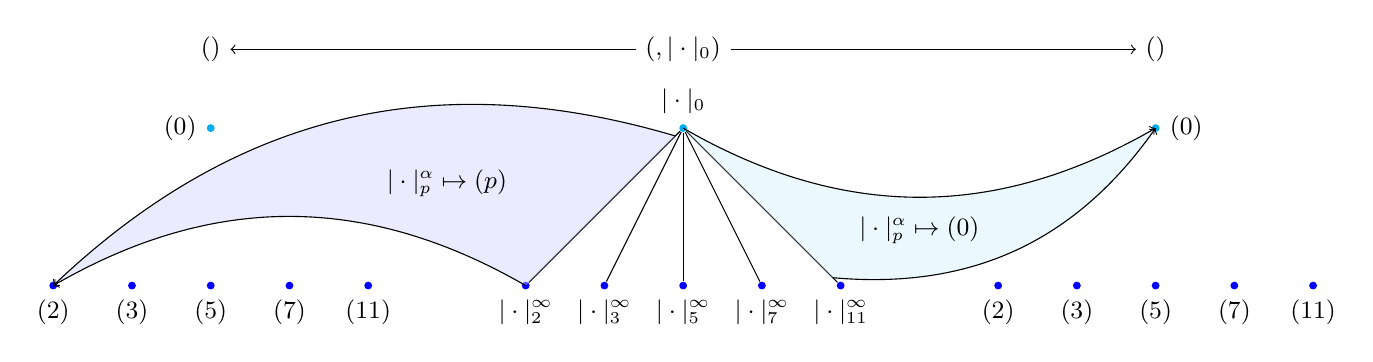
\begin{tikzpicture}[scale=1, every node/.style={font=\small}]
            % M(Z) points
            \node (MZ) at (0,1) {\(\scrM(\bbZ, |\cdot|_0)\)};
            %% trivial norm (root)
            \node[circle, fill=cyan,inner sep=1pt, label=above:{\(|\cdot|_0\)}] (root) at (0,0) {};
            %% non-archimedean branches
            \foreach \p/\n in {2/1,3/2,5/3,7/4,11/5} {
                \node[circle, fill=blue, inner sep=1pt, label=below:{\(|\cdot|_{\p}^\infty\)}] (p_top_\p) at (-3 + \n,-2) {};
                \draw (root) -- (p_top_\p);
            }

            % Spec(Z) points, left side
            \node (SpecZ_left) at (-6,1) {\(\Spec(\bbZ)\)};
            %% generic point
            \node[circle, fill=cyan,inner sep=1pt, label=left:{\((0)\)}] (root) at (-6,0) {};
            %% special points
            \foreach \p/\n in {2/1,3/2,5/3,7/4,11/5} {
                \node[circle, fill=blue, inner sep=1pt, label=below:{\((\p)\)}] (p_top_\p) at (-9 + \n,-2) {};
                % \draw (root) -- (p_top_\p);
            }

            % Spec(Z) points, right side
            \node (SpecZ_right) at (6,1) {\(\Spec(\bbZ)\)};
            %% generic point
            \node[circle, fill=cyan,inner sep=1pt, label=right:{\((0)\)}] (root) at (6,0) {};
            %% special points
            \foreach \p/\n in {2/1,3/2,5/3,7/4,11/5} {
                \node[circle, fill=blue, inner sep=1pt, label=below:{\((\p)\)}] (p_top_\p) at (3 + \n,-2) {};
                % \draw (root) -- (p_top_\p);
            }

            % map arrows
            \draw[->] (MZ) -- (SpecZ_left) node[midway, above] {\(\Red\)};
            \draw[->] (MZ) -- (SpecZ_right) node[midway, above] {\(\Ker\)};

            % reduction map, maps to closed points
            \fill[blue!20,opacity=0.4] (-0.1,-0.1) to[bend right] (-8,-2) to[bend left] (-2,-2) -- cycle;
            \draw[->] (-0.1,-0.1) to[bend right] (-8,-2);
            \draw[->] (-2,-2) to[bend right] (-8,-2);
            \node at (-3,-0.7) {\(|\cdot|_p^\alpha \mapsto (p)\)};

            % kernel map, maps to generic point
            \fill[cyan!20,opacity=0.4] (0,0) to[bend right] (6,0) to[bend left] (1.9,-1.9) -- cycle;
            \draw[->] (0,0) to[bend right] (6,0);
            \draw[->] (1.9,-1.9) to[bend right] (6,0);
            \node at (3,-1.3) {\(|\cdot|_p^\alpha \mapsto (0)\)};
        \end{tikzpicture}
        \end{center}
        % \Yang{To be continued.}
    \end{example}

    \begin{proposition}\label{prop:reduction_map_inverse_open_subset_to_closed_subset}
        Let \(R\) be a non-archimedean Banach ring and \(\widetilde{U} \subset \Spec(\widetilde{R})\) be a Zariski open subset.
        Then the preimage \(\Red^{-1}(\widetilde{U})\) is a closed subset of \(\scrM(R)\).
    \end{proposition}
    \begin{proof}
        \Yang{To be completed.}
    \end{proof}


\subsection{Spectrum of Tate algebras}

    \paragraph{Spectrum of Tate algebra in one variable} Let \(\kkk\) be an algebraically closed complete non-archimedean field, and let \(A = \kkk\{T/r\}\).
    We list some types of points in the spectrum \(\scrM(A)\).

    \begin{construction}\label{cons:four_types_of_points_in_spectrum_of_Tate_algebra_in_one_variable}
        For each \(a \in \kkk\) with \(|a| \leq r\), we have the \emph{type I} point \(x_a\) corresponding to the evaluation at \(a\), i.e., \(|f|_{x_a} := |f(a)|\) for each \(f \in A\).
        
        For each closed disk \(E = E(a,s) := \{b \in \kkk : |b - a| \leq s\}\) with center \(a \in \kkk\) and radius \(s \leq r\), we have the point \(x_E = x_{a,s}\) corresponding to the multiplicative semi-norm defined by
        \[ |f|_{x_E} = |f|_{x_{a,s}} := \sup_{b \in E(a,s)} |f(b)| \]
        for each \(f \in A\).
        If \(s \in |\kkk^\times|\), then the point \(x_E\) is called a \emph{type II} point; otherwise, it is called a \emph{type III} point.
        
        Let \(E_n = E(a_n,s_n)\) be a sequence of closed disks in \(\kkk\) such that \(E_{n+1} \subsetneq E_n\) and \(\bigcap_n E_n = \emptyset\).
        Then we have the point \(x_{\{E_n\}} = x_{\{a_n,s_n\}}\) corresponding to the multiplicative semi-norm defined by
        \[ |f|_{x_{\{E_n\}}} = |f|_{x_{\{a_n,s_n\}}} := \inf_n |f|_{x_{E_n}} \]
        for each \(f \in A\).
        Such a point is called a \emph{type IV} point.
        \Yang{To be completed. Check the definition of type IV points.}
    \end{construction}
    % \end{example}

    \begin{proposition}\label{prop:four_types_of_points_in_spectrum_of_Tate_algebra_in_one_variable}
        The points in the spectrum \(\scrM(\kkk\{r^{-1}T\})\) can be classified into four types as described above.
        % \Yang{To be checked}
    \end{proposition}
    \begin{proof}
        Fix \(x \in \scrM(\kkk\{r^{-1}T\})\), set 
        \[ s = \inf_{a \in \kkk} |T - a|_x \leq r,\quad  E = \{a \in \kkk : |T - a|_x = s\} \subset E(0,r). \]

        \begin{case}\label{case_in_proof_of_four_type_points:point_type_I}
            \(E \neq \emptyset\) and \(s=0\). 
        \end{case}
        By assumption, there exists \(a \in E\) such that \(|T - a|_x = 0\).
        Note that if \(f(a) = 0\), then \(T-a \mid f\) in \(\kkk\{r^{-1}T\}\) and hence \(|f|_x = |T - a|_x|g|_x = 0\).
        Then we have 
        \[ |f(a)| = \big| |f(a)| - |f(a) - f|_x \big| \leq |f|_x \leq |f(a)| + |f(a) - f|_x = |f(a)| \]
        for each \(f \in \kkk\{r^{-1}T\}\), which implies that \(|f|_x = |f(a)|\).
        Thus \(x\) is a type I point \(x_a\).

        \begin{case}\label{case_in_proof_of_four_type_points:point_type_II_and_III}
            \(E \neq \emptyset\) and \(s > 0\).
        \end{case}
        % Next suppose that \(E \neq \emptyset\) and \(s > 0\).
        Let \(a \in E\).
        Note that for every \(b \in \kkk\), we have 
        \[ |a-b| \leq \max\{|T - a|_x, |T - b|_x\} = |T - b|_x. \]
        First we show that \(E = E(a,s)\).
        For each \(b \in E(a,s)\), we have \(|T - b|_x \leq \max\{|T - a|_x, |a - b|\} = s\), which implies that \(b \in E\).
        Conversely, for each \(b \in E\), we have \(|a - b| \leq \max\{|T - a|_x, |T - b|_x\} = s\).

        Let \(f \in \kkk[T]\) be a polynomial.
        Write \(f = \prod_{i=1}^n (T - c_i)\) for some \(c_1, \ldots, c_n \in \kkk\).
        Then we have
        \[ |f|_x = \prod_{i=1}^n |T - c_i|_x \geq \prod_{i=1}^n |b - c_i| = |f(b)|, \quad \forall b \in E. \]
        I claim that for every \(\varepsilon \in (0,1)\), there exists \(b \in E\) such that \(\varepsilon |T-c_i|_x < |b - c_i|\) for each \(i = 1, \ldots, n\).
        Indeed, if \(c_i \notin E\), then \(|T-c_i|_x = |b - c_i|\) for each \(b \in E\).
        Hence we only need to consider the case when \(c_i \in E\).
        Since \(\kkk\) is algebraically closed, \(E(a,s) \setminus \bigcup_{i=1}^n E(c_i,\varepsilon s) \neq \emptyset\).
        Choose \(b\) in the set.
        Then we have 
        \[ |f(b)| \geq \prod_{i=1}^n \varepsilon |T - c_i|_x = \varepsilon^n |f|_x. \]
        Thus \(|f|_x = \sup_{b \in E} |f(b)|\) for each polynomial \(f \in \kkk[T]\).
        Since polynomials are dense in \(\kkk\{r^{-1}T\}\), we have \(|f|_x = \sup_{b \in E} |f(b)|\) for each \(f \in \kkk\{r^{-1}T\}\).
        Therefore, \(x\) is the point \(x_E = x_{a,s}\), which is of type II or type III depending on whether \(s \in |\kkk^\times|\) or not.

        \begin{case}\label{case_in_proof_of_four_type_points:point_type_IV}
            \(E = \emptyset\).
        \end{case}

        Set \(E_n = \{a \in \kkk : |T - a|_x \leq s + 1/n\}\) and \(a_n \in E_n\) for each \(n \in \bbN\).
        By the similar argument as in \cref{case_in_proof_of_four_type_points:point_type_II_and_III}, we have \(E_n = E(a_n, s + 1/n)\).
        Note that \(E_n\) is a decreasing sequence of closed disks with \(\bigcap_n E_n = E = \emptyset\).
        
        For \(c \in \kkk\), there exists \(N\) such that \(\forall n \geq N\), we have
        \[ c \notin E_n \implies |T - c|_x > |T - a_n|_x \implies |T - c|_x = |a_n - c|. \]
        Thus
        \[ \inf_n |T-c|_{E_n} = \inf_n |a_n - c| = |T - c|_x. \]
        By multiplicativity, we have \(\inf_n |f|_{E_n} = |f|_x\) for each polynomial \(f \in \kkk[T]\).
        And then by density of polynomials, the equality holds for each \(f \in \kkk\{r^{-1}T\}\).
        Therefore, \(x = x_{\{E_n\}} = x_{\{a_n,s_n\}}\) is of type IV.
        % \Yang{To be completed.}
    \end{proof}

    \begin{proposition}\label{prop:the_complete_residue_field_of_all_four_types_points_in__spectrum_of_Tate_algebra_in_one_variable}
        The completed residue fields of the four types of points in the spectrum \(\scrM(\kk\{r^{-1}T\})\) are described as follows:
        \begin{itemize}
            \item type I point \(x_a\): \(\scrH(x_a)\) is isomorphic to \(\kkk\);
            \item type II point \(x_{a,s}\): \(\scrH(x_{a,s}) \cong \calk_\kkk((t))\);
            \item type III point \(x_{a,s}\): \(\calk_{\scrH(x_{a,s})} \cong \calk_\kkk\) and the value group \(|\scrH(x_{a,s})^\times|\) is generated by \(|\kkk^\times|\) and \(s\);
            \item type IV point \(x_{\{a_n,s_n\}}\): \(\scrH(x_{\{a_n,s_n\}})\) is an immediate extension of \(\kkk\).
        \end{itemize}
        \Yang{To be checked.}
    \end{proposition}
    \begin{proof}
        \Yang{To be completed.}
    \end{proof}

    \begin{example}\label{eg:completed_residue_field_of_type_III_and_IV_points_in_spectrum_of_Tate_algebra_in_one_variable}
        The completed residue field \(\scrH(x_a)\) for a type I point \(x_a\) with \(a \in \kkk\) and \(|a| \leq r\) is isomorphic to \(\kkk\).
        \Yang{To be complete.}
    \end{example}

    \begin{example}\label{eg:Tate_algebra_in_1_variable_under_reduction_map}
        Let \(\kkk\) be a complete algebraically closed non-archimedean field and \(A = \kkk\{T/r\}\).
        We have \(\widetilde{A} \cong \calk_\kkk[T]\).
        For a point \(x_a \in \scrM(A)\) of type I corresponding to \(a \in \kkk\) with \(|a| \leq r\) (see \cref{cons:four_types_of_points_in_spectrum_of_Tate_algebra_in_one_variable}), 
        the induced homomorphism \(\widetilde{A} = \calk_\kkk[T] \to \calk_{\scrH(x_a)} = \calk_\kkk\) is given by \(T \mapsto a \mod \kkk^{\circ \circ}\).

        \Yang{To be continued.}
    \end{example}

    \paragraph{Spectrum of Tate algebra in servel variables} Let \(\kkk\) be a complete non-archimedean field, and let \(A = \kkk\{r_1^{-1}T_1, \ldots, r_n^{-1}T_n\}\).
    We can consider the spectrum \(\scrM(A)\) similarly.